\chapter{Określenie wymagań oraz projekt graficzny systemu}

\section{Wymagania funkcjonalne}
System ma współpracować z już istniejącym oprogramowaniem Dispatch Rider. W tym celu podjęliśmy się zdefiniowania następujących wymagań funkcjonalnych takich jak:

\begin{enumerate}
	\item Generowanie plików konfiguracyjnych dla Dispatch Ridera:
		\begin{itemize}
			\item generowanie pliku określającego zlecenia, o składni:
			\textbf{ilość-pojazdów ładowność prędkość}
			\item generowanie pliku określającego czas nadchodzenia zleceń, o składni: nr-lini \textbf{czas-zlecenia}
			\item generowanie pliku zawierającego liczbę kierowców
			\item generowanie pliku określającego parametry ciągników, o składni: \textbf{moc niezawodność wygoda zużycie-paliwa typ-zaczepu}
			\item generowanie pliku opisującego parametry naczep o składni: \textbf{masa pojemność typ-ładunku uniwersalność typ-zaczepu}
			\item generowanie pliku opisującego parametry holonów o składni: initialCapacity = \textbf{pojemność-pojazdu} mode = \textbf{tryb} bases = \textbf{ilość-baz} eUnitsCount = \textbf{ilość-jednostek}
			\item generowanie pliku konfiguracyjnego configuration.xml
		\end{itemize}
		
	\item Kolejkowanie zadań zlecanych systemowi.
	
	\item Uruchamianie systemu Dispatch Rider z użyciem dostarczonych z zewnątrz lub wygenerowanych plików
	
	\item Odczyt i parsowanie plików wynikowych Dispatch Ridera, wraz z wizualizacją otrzymanych wyników
		\begin{itemize}
			\item wizualizacja grafu sieci transportowej
			\item wizualizacja tras pokonanych przez pojazdy
			\item wyświetlanie informacji o każdym z holonów 
			\item wyświetlanie zbiorczego podsumowania obliczeń zawierającego koszt, dystans, czas, parametry holonów
		\end{itemize}
	\item Przechowywanie wyników obliczeń, w celu zaprezentowania na żądanie
\end{enumerate}

\section{Wymagania niefunkcjonalne}

\begin{enumerate}
	\item Bezpieczeństwo zapewniane poprzez autoryzację użytkowników.
    \item Dokumentacja techniczna w postaci strony wiki, dokumentu tekstowego oraz komentarzy w kodzie programu.
    \item Przenośność - zapewnienie w pełni poprawnego działania programu na najpopularniejszych przeglądarkach oraz systemach operacyjnych.
    \item Płynność działania wizualizacji grafów w oknie przeglądarki.
    \item Łatwość i intuicyjność obsługi, umożliwienie komfortowego korzystania z programu bez poznawania szczegółowych instrukcji dotyczących uruchamiania i konfiguracji.
\end{enumerate}
\section{Projekt GUI}
Projektując GUI webowe staraliśmy się zmaksymalizować czytelność i łatwość korzystania z naszej aplikacji. W związku z tym chcielibyśmy zaimplementować wygląd aplikacji w taki sposób, by informacje w danym momencie nieistotne nie przysłaniały użytkownikowi tych, na których chciałby się skupić. Poniżej prezentujemy pierwsze szkice, które stworzyliśmy. 
\begin{center}
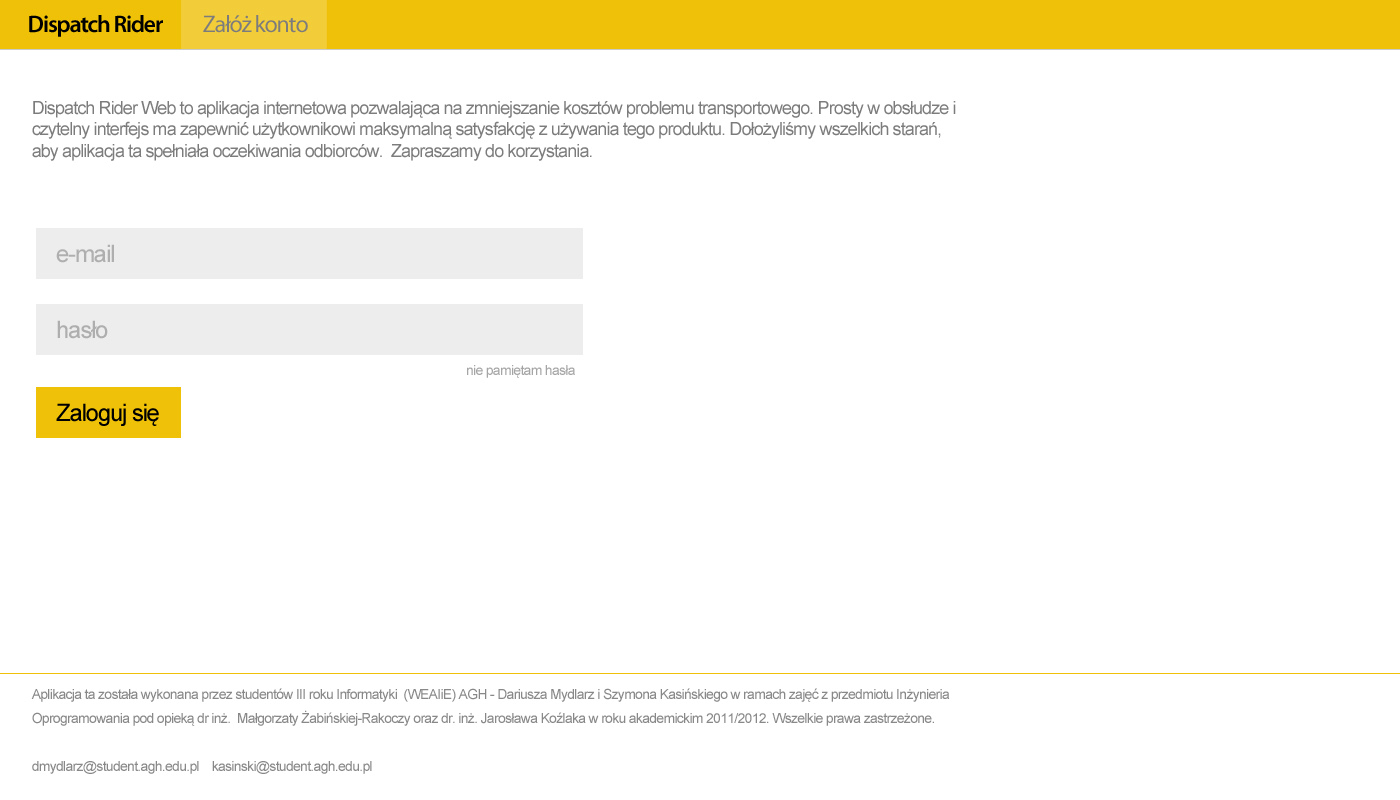
\includegraphics[scale=0.3]{imgs/unlogged_home.jpg}

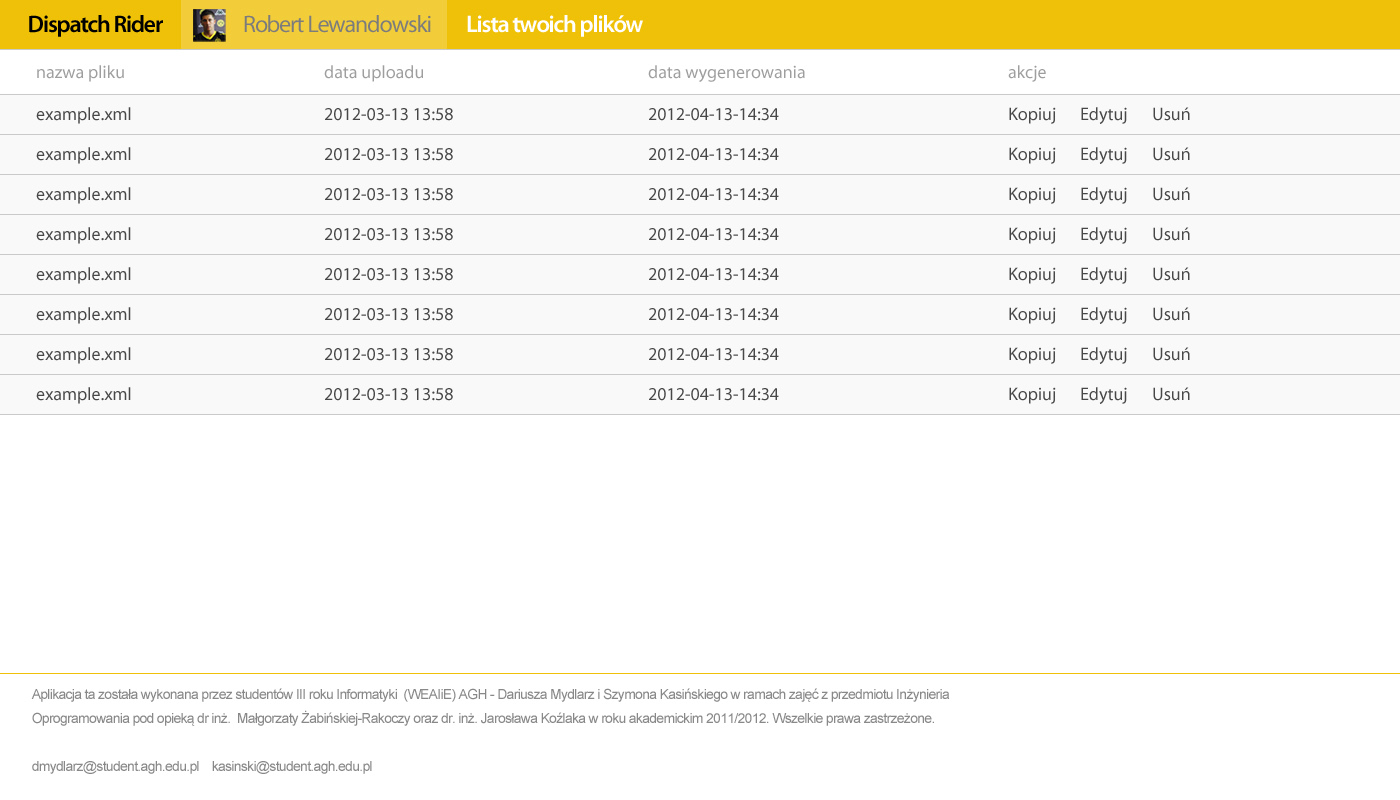
\includegraphics[scale=0.3]{imgs/logged_home.jpg}

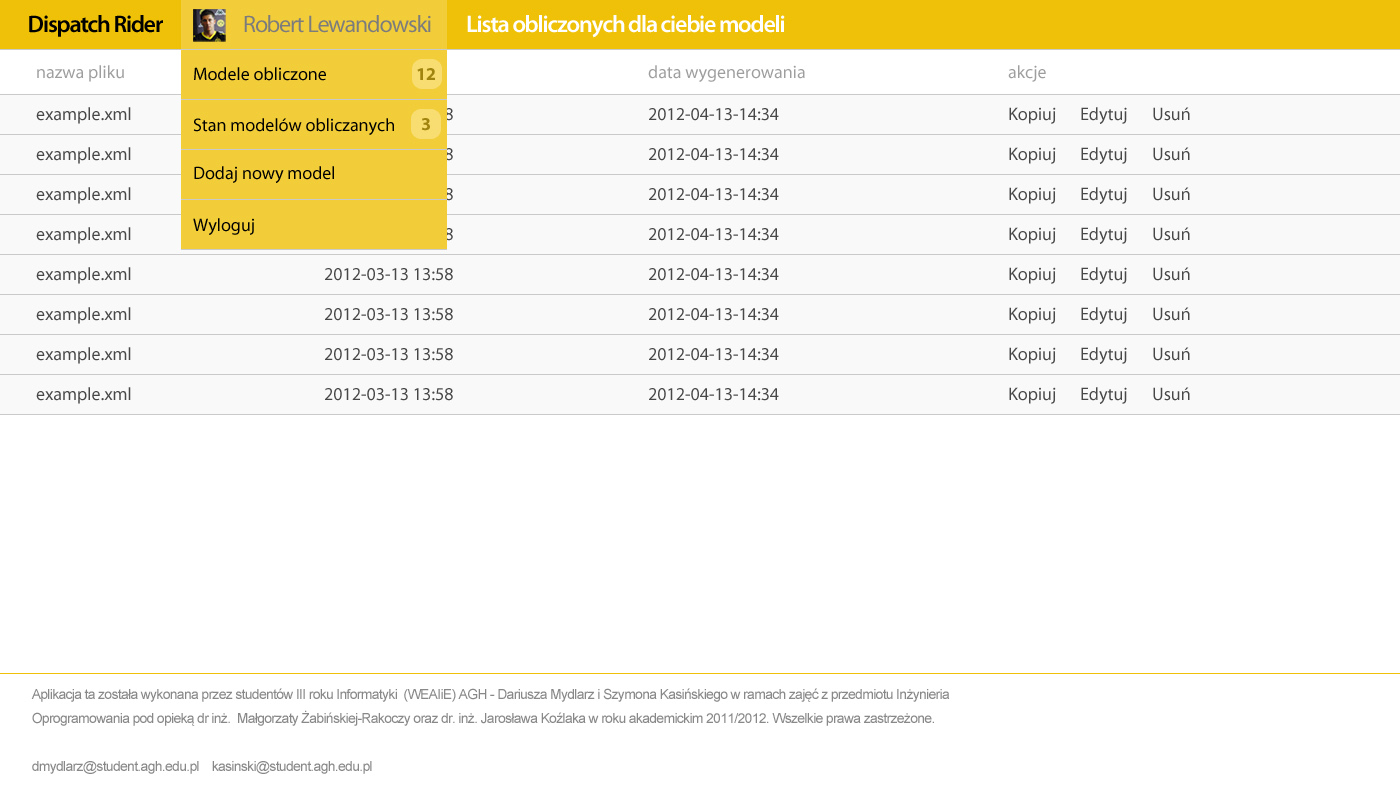
\includegraphics[scale=0.3]{imgs/logged_home_menu.jpg}

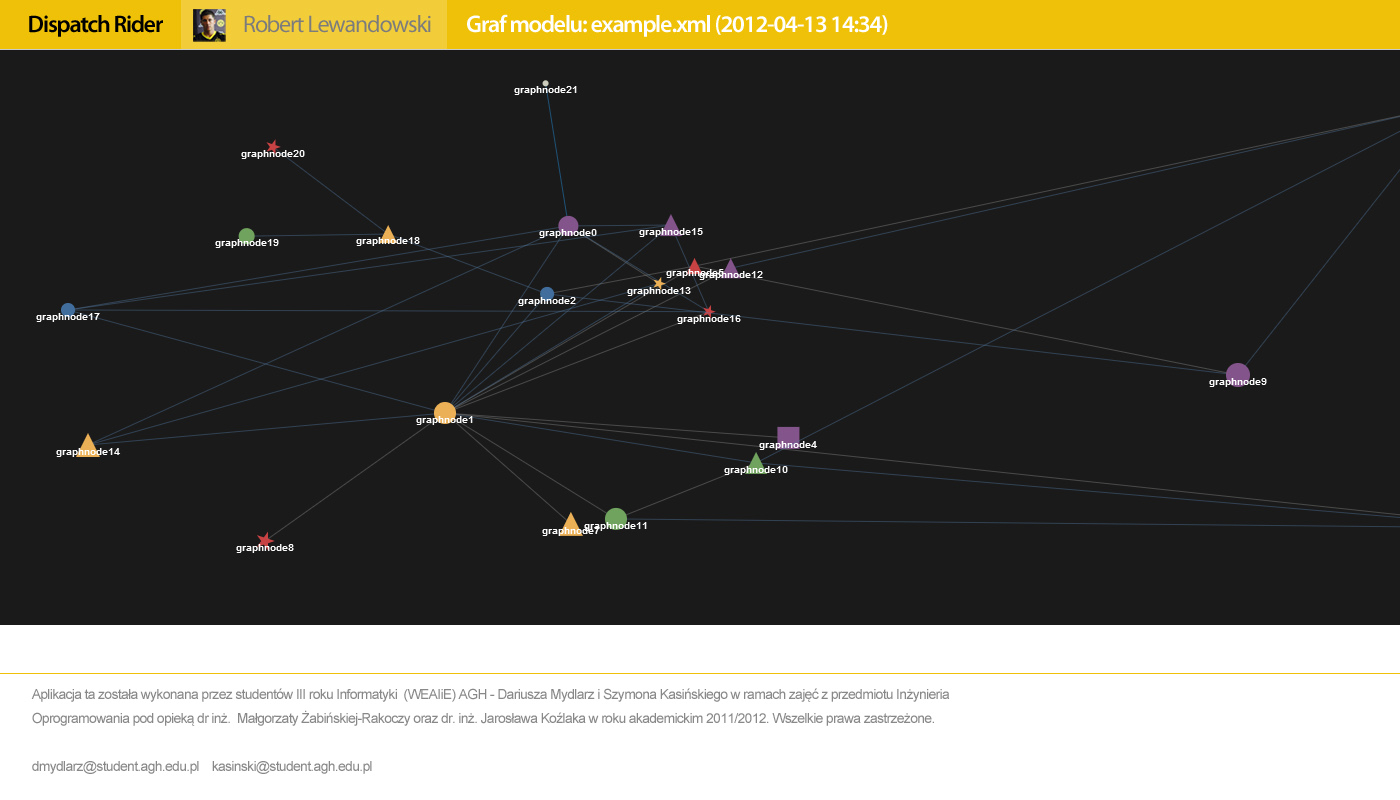
\includegraphics[scale=0.3]{imgs/logged_graph_viewjpg.jpg}
\end{center}
